\documentclass[12pt,twoside]{report}

% PACKAGES
\usepackage{graphicx}
\usepackage{caption}
\usepackage{subcaption}
\usepackage[a4paper,width=150mm,top=25mm,bottom=25mm,bindingoffset=6mm]{geometry}
\usepackage{fancyhdr}
\usepackage{parskip}
\usepackage[square,numbers]{natbib}
\usepackage[unicode]{hyperref}
\usepackage{amsmath}
\usepackage[acronym]{glossaries}
\usepackage{lipsum} %DUMMY TEXT

% CONFIGS
\pagestyle{fancy}
\setlength{\headheight}{14.49998pt}
\fancyhead{}
\fancyhead[RO,LE]{Evaluasi Pengalaman Pengguna Digilib IIB Darmajaya Menggunakan UEQ}    % TODO: CHANGE THIS
\fancyfoot{}
\fancyfoot[LO,CE]{\ifnum\value{chapter}=0 \else \leftmark \fi}
\fancyfoot[LE,RO]{\thepage}
\hypersetup{
    pdfauthor = {Steven Erlinto}, % TODO: CHANGE THIS
    pdftitle = {Evaluasi Pengalaman Pengguna Digilib IIB Darmajaya Menggunakan UEQ}, % TODO: CHANGE THIS
    colorlinks,
    linkcolor={blue},
    citecolor={blue}
}

% MACROS
% essentials 
\renewcommand{\headrulewidth}{0.4pt}
\renewcommand{\footrulewidth}{0.4pt}
% non-essentials (some examples)
\newcommand{\unit}[1]{\ensuremath{\, \mathrm{#1}}}  % makes writing units simpler
\renewcommand{\thefootnote}{\emph{\alph{footnote}}} % italic letters footnote

% PATHS
\graphicspath{ {img/} }
\makeglossaries

\newacronym{ueq}{UEQ}{User Experience Questionnaire}
\newacronym{ui}{UI}{User Interface}
\newacronym{ux}{UX}{User Experience}
\newacronym{digilib}{Digilib}{Digital Library}

% BIB SETUP
\bibliographystyle{ieeetr} % Cite style (natbib is better)


% <><><><><><><><><><><><><><><><><><><><><><>
% DOCUMENT BEGIN HERE
\begin{document}

\begin{titlepage}
    \begin{center}
        \vspace*{1cm}
        
        \Huge
        \textbf{Deteksi Wajah Menggunakan Metode Euclidian Distance}
        
        \vspace{1.5cm}
        
        Adi Wicaksono
        
        \vfill

        \large
        Diajukan Sebagai Salah Satu Syarat untuk Mencapai Gelar\\
        SARJANA KOMPUTER\\
        Pada Program Studi Teknik Informatika\\
        IIB Darmajaya Bandar Lampung \\
        
        
        \vspace{0.8cm}
        
        
\includegraphics[width=0.4\textwidth]{darmajaya.jpg}
        
        \large
        Program Studi Teknik Informatika\\
        Fakultas Ilmu Komputer\\
        Institut Informatika dan Bisnis Darmajaya\\
        Indonesia\\
        \today

        \vfill

        {\Large Supervisor: Dr. \;Muhammad Said Hasibuan} \\ \, \\
       
       
        
    \end{center}
\end{titlepage}
\lipsum[1-3]
pada hari
\pagenumbering{gobble}
\chapter*{Dedication}
Skripsi ini didekasikan
\chapter*{Declaration}
\lipsum[1-3]
\input{mis/acknowledgements}

\tableofcontents
\listoffigures
\listoftables
\printglossary[type=\acronymtype]

\chapter{Pendahuluan}\label{cha:intro}

Di era digitalisasi pendidikan modern (berdasarkan standar ISO 9241-210 \cite{iso2019ergonomics} mengenai interaksi manusia dan sistem), keberadaan perpustakaan digital (\gls{digilib}) telah menjadi tulang punggung aktivitas akademik mahasiswa. Bagi institusi pendidikan tinggi seperti IIB Darmajaya, platform \gls{digilib} bukan sekadar gudang repositori jurnal atau skripsi, melainkan pusat interaksi literatur ilmiah. Sayangnya, banyak pengembangan platform akademik yang masih terlalu berfokus pada kelengkapan fitur teknis di \textit{back-end}, namun mengabaikan aspek kenyamanan pengguna (\gls{ux}) di \textit{front-end}. Akibatnya, antarmuka yang membingungkan atau alur pencarian referensi yang berbelit-belit seringkali membuat mahasiswa enggan memanfaatkan layanan ini secara maksimal dan lebih memilih mencari referensi di platform eksternal.

Penelitian-penelitian terdahulu mengenai evaluasi sistem informasi perpustakaan seringkali masih bertumpu pada pengujian fungsionalitas dasar (\textit{usability testing}) atau menggunakan kuesioner kepuasan layanan yang konvensional. Metode evaluasi tradisional ini memiliki kelemahan mendasar, yakni hanya mengukur apakah sebuah sistem "berfungsi dan bisa digunakan", tanpa menilai secara mendalam bagaimana perasaan atau pengalaman subjektif pengguna saat berinteraksi dengan sistem tersebut. Sebuah aplikasi yang bebas dari \textit{error} sistem (\textit{bug}) belum tentu memberikan pengalaman yang menyenangkan atau memotivasi penggunanya. Di sisi lain, beberapa metode survei evaluasi \gls{ux} seringkali terlalu panjang dan kompleks, sehingga menyulitkan proses pengumpulan data yang objektif dari responden mahasiswa.

Merespons keterbatasan tersebut, penelitian ini mengusulkan pendekatan evaluasi menyeluruh menggunakan kerangka kerja \gls{ueq} \cite{schrepp2014applying}. Jika evaluasi konvensional hanya melihat aspek pragmatis, pendekatan \gls{ueq} dalam penelitian ini dirancang untuk membedah interaksi pengguna secara komprehensif melalui enam dimensi metrik: \textit{Attractiveness} (daya tarik), \textit{Perspicuity} (kejelasan), \textit{Efficiency} (efisiensi), \textit{Dependability} (ketepatan), \textit{Stimulation} (stimulasi), dan \textit{Novelty} (kebaruan). Pemilihan metode \gls{ueq} didasarkan pada keunggulannya sebagai alat ukur terstandarisasi yang mampu menyeimbangkan aspek kualitas fungsional (pragmatis) dan aspek emosional (hedonis) secara cepat dan reliabel dengan metode analisis kuantitatif.

Kontribusi utama penelitian ini terletak pada dua aspek strategis: (1) Penerapan pengukuran \gls{ux} yang komprehensif untuk mendeteksi secara presisi titik-titik kelemahan desain (\textit{pain points}) pada antarmuka \gls{digilib} IIB Darmajaya tanpa bergantung pada asumsi pengembang semata; dan (2) Penyediaan landasan evaluasi dan rekomendasi perbaikan berbasis data (\textit{data-driven}) yang konkret bagi pengelola sistem informasi kampus, sehingga perombakan sistem di masa depan dapat lebih terarah dalam menciptakan ekosistem akademik digital yang ramah pengguna.
\pagenumbering{arabic}
\chapter{Tinjauan Pustaka}\label{cha:litreivew}

\section{Perpustakaan Digital (Digital Library)}
Perpustakaan digital adalah sistem informasi yang mengumpulkan, mengelola, dan menyediakan akses ke koleksi digital berupa jurnal, buku, skripsi, dan karya ilmiah lainnya melalui jaringan internet \cite{arms2001digital}. Kehadiran perpustakaan digital di institusi pendidikan mempermudah sivitas akademika dalam mencari referensi tanpa batasan ruang dan waktu \cite{pendit2008perpustakaan}. Penggunaannya sangat bergantung pada kualitas antarmuka dan kemudahan navigasi agar informasi dapat ditemukan secara cepat, tepat, dan akurat oleh pengguna \cite{saleh2020manajemen}.

\section{Sistem Informasi Akademik}
Sistem informasi akademik merupakan integrasi perangkat keras dan perangkat lunak yang dirancang untuk mendukung proses manajemen dan layanan pendidikan di perguruan tinggi \cite{jogiyanto2005analisis}. Layanan ini berfokus pada penyampaian informasi yang efisien kepada mahasiswa dan dosen. Kualitas platform akademik yang baik tidak hanya dinilai dari kelengkapan fiturnya, tetapi juga dari seberapa baik sistem tersebut memenuhi ekspektasi penggunanya dalam menyelesaikan tugas-tugas pencarian literatur \cite{delone2003delone}.

\section{User Interface (UI)}
\gls{ui} adalah bagian visual dari sistem perangkat lunak yang menjadi titik interaksi langsung antara pengguna dan komputer. Desain \gls{ui} mencakup elemen tata letak, warna, tipografi, serta komponen interaktif seperti tombol, kolom pencarian, dan menu navigasi \cite{tidwell2010designing}. Desain \gls{ui} yang baik harus intuitif, terstruktur, dan konsisten sehingga dapat meminimalkan kesalahan pengguna saat mengoperasikan sistem \cite{galitz2007essential}. Antarmuka yang rumit dan tidak terorganisir seringkali menjadi penyebab utama pengguna meninggalkan sebuah platform digital \cite{setiawan2023implementasi}.

\section{User Experience (UX)}
\gls{ux} mencakup seluruh persepsi, emosi, dan respons pengguna yang muncul sebelum, selama, dan setelah berinteraksi dengan sebuah produk atau sistem \cite{iso2019ergonomics}. Berbeda dengan \gls{ui} yang berfokus pada tampilan visual, \gls{ux} lebih menitikberatkan pada alur operasional, kenyamanan, dan nilai yang dirasakan pengguna saat mencapai tujuannya \cite{hassenzahl2006user}. \gls{ux} yang optimal akan menciptakan pengalaman yang mulus (\textit{seamless}), mengurangi hambatan kognitif (\textit{cognitive load}), dan pada akhirnya meningkatkan motivasi pengguna untuk terus menggunakan sistem \cite{garrett2011elements}.

\section{Desain Interaksi}
Desain interaksi berfokus pada penciptaan dialog yang bermakna antara pengguna dan sistem digital \cite{preece2015interaction}. Prinsip ini memastikan bahwa setiap tindakan pengguna, seperti mengunduh dokumen atau melakukan pencarian referensi, mendapatkan umpan balik (\textit{feedback}) yang jelas dari sistem. Penerapan desain interaksi yang baik dalam perpustakaan digital akan membantu pengguna memahami arsitektur informasi dan hierarki data dengan lebih cepat tanpa memerlukan panduan manual yang rumit \cite{cooper2014about}.

\section{Kepuasan Pengguna (User Satisfaction)}
Kepuasan pengguna adalah respons emosional yang timbul ketika sebuah sistem berhasil memenuhi atau melampaui harapan pengguna dalam menyelesaikan suatu tugas \cite{bhattacherjee2001understanding}. Dalam konteks layanan digital kampus, faktor-faktor seperti kecepatan akses, relevansi hasil pencarian, dan kemudahan pengunduhan sangat memengaruhi tingkat kepuasan \cite{mulyadi2023analisis}. Pengguna yang merasa puas cenderung akan terus menggunakan layanan \gls{digilib} tersebut sebagai sumber referensi utama mereka.

\section{User Experience Questionnaire (UEQ)}
\gls{ueq} adalah instrumen evaluasi terstandarisasi yang digunakan untuk mengukur pengalaman pengguna secara komprehensif, cepat, dan reliabel \cite{schrepp2014applying}. Kuesioner ini mengukur kualitas pragmatis (fungsionalitas) dan kualitas hedonis (emosional) pengguna melalui 26 item pertanyaan. Evaluasi ini terbagi dalam 6 dimensi: \textit{attractiveness} (daya tarik), \textit{perspicuity} (kejelasan), \textit{efficiency} (efisiensi), \textit{dependability} (ketepatan), \textit{stimulation} (stimulasi), dan \textit{novelty} (kebaruan). Skala penilaiannya berkisar dari -3 (sangat negatif) hingga +3 (sangat positif), memungkinkan peneliti untuk melakukan evaluasi kuantitatif (\textit{benchmark}) atas persepsi pengguna terhadap produk digital secara menyeluruh.
\chapter{Metode Penelitian}\label{cha:method}

\section{Populasi}
Populasi sasaran dalam penelitian ini adalah mahasiswa aktif IIB Darmajaya yang pernah atau rutin menggunakan layanan perpustakaan digital (\gls{digilib}) IIB Darmajaya. Jumlah pastinya tidak dapat diketahui secara pasti, sehingga populasi ditetapkan berdasarkan kriteria pengguna aktif platform tersebut. Pengguna yang dijadikan subjek penelitian merupakan mahasiswa yang telah menggunakan \gls{digilib} IIB Darmajaya untuk berbagai keperluan akademik, seperti pencarian jurnal, buku referensi, maupun skripsi, dengan durasi penggunaan yang bervariasi. Pengguna tersebut terdiri dari mahasiswa yang rutin mengakses layanan untuk tugas perkuliahan sehari-hari maupun yang menggunakan secara insidentil saat penyusunan tugas akhir. Objek dalam penelitian ini adalah platform \gls{digilib} IIB Darmajaya, khususnya pada aspek \gls{ui}/\gls{ux}, dengan tujuan untuk mengevaluasi pengalaman pengguna serta mengidentifikasi area antarmuka yang perlu dioptimalkan.

\section{Sampel}
Sampel dalam penelitian ini berjumlah 40 responden yang dipilih menggunakan teknik \textit{purposive sampling}, yaitu metode penentuan sampel berdasarkan kriteria tertentu yang sesuai dengan kebutuhan studi (dalam hal ini mahasiswa IIB Darmajaya yang memiliki pengalaman mengakses \gls{digilib}). Pemilihan teknik ini bertujuan untuk memastikan bahwa responden memiliki pengalaman relevan terhadap objek yang dikaji. Penetapan jumlah responden mengacu pada pedoman \gls{ueq}, di mana rentang 20 hingga 30 responden dianggap memadai untuk memperoleh data yang stabil \cite{schrepp2014applying}. Jumlah ditetapkan sebanyak 40 responden guna meminimalkan potensi bias dan meningkatkan akurasi hasil analisis. Dari jumlah tersebut, sebanyak 5 responden dipilih untuk diwawancarai lebih lanjut guna memperoleh data kualitatif yang lebih mendalam terkait keluhan dan pengalaman penggunaan platform.

\section{Teknik Model Analisis}
Penelitian ini menggunakan metode campuran (\textit{mixed method}) dengan dominasi pendekatan kuantitatif sebesar 70\% dan kualitatif sebesar 30\%. Teknik analisis data dilakukan secara bertahap mulai dari pengumpulan data, pembuatan solusi desain, hingga evaluasi akhir menggunakan metode \gls{ueq} dan pendekatan Lean UX. Analisis kuantitatif dilakukan menggunakan kuesioner \gls{ueq} yang dianalisis melalui perangkat \textit{UEQ Analysis Tool} berbasis Microsoft Excel untuk mengukur enam skala pengalaman pengguna. Analisis kualitatif melengkapi proses ini melalui observasi, wawancara, dan \textit{usability testing}. Teknik analisis data dalam penelitian ini melibatkan beberapa tahapan utama sebagai berikut:

\begin{enumerate}
    \item \textbf{Pengumpulan Data Awal:}
    Menggunakan studi literatur, observasi langsung pada antarmuka pengguna \gls{digilib} IIB Darmajaya, survei \textit{online} (penyebaran kuesioner \gls{ueq} kepada 40 responden mahasiswa), dan wawancara mendalam terhadap 5 responden yang dipilih menggunakan \textit{convenience sampling}.
    
    \item \textbf{Analisis Awal:}
    Data kuantitatif dari kuesioner \gls{ueq} dianalisis secara deskriptif menggunakan \textit{Data Analysis Tool}, lalu dibandingkan dengan \textit{benchmark} \gls{ueq} untuk mengidentifikasi aspek \gls{ui}/\gls{ux} dari \gls{digilib} yang bernilai rendah dan perlu ditingkatkan.
    
    \item \textbf{Perancangan Solusi:}
    Berdasarkan temuan data dan keluhan pengguna, peneliti menyusun dugaan masalah (\textit{declare assumption}) dan membuat perancangan ulang antarmuka dalam bentuk \textit{Minimum Viable Product} (MVP) menggunakan perangkat lunak Figma, mulai dari \textit{wireframe} hingga \textit{high-fidelity prototype}.
    
    \item \textbf{Eksperimen dan Validasi:}
    Prototipe desain antarmuka \gls{digilib} yang baru diuji melalui \textit{usability testing} (misalnya menggunakan platform Maze atau pengujian prototipe langsung) serta diukur kembali menggunakan kuesioner \gls{ueq} untuk melihat perbedaan skor pengalaman pengguna sebelum dan sesudah perbaikan desain.
    
    \item \textbf{Evaluasi Akhir:}
    Hasil \gls{ueq} akhir pada prototipe desain dibandingkan dengan hasil awal (sistem \gls{digilib} saat ini) untuk menilai tingkat keberhasilan rancangan dalam meningkatkan kenyamanan dan pengalaman pengguna aplikasi \gls{digilib} IIB Darmajaya.
\end{enumerate}
\chapter{Hasil dan Pembahasan}\label{cha:result}

Dalam penelitian ini, analisis statistik deskriptif dilakukan dengan menghitung nilai rata-rata (\textit{mean}) dari setiap item pada skala kuesioner untuk memperoleh pemahaman mengenai persepsi mahasiswa terhadap kualitas antarmuka platform \gls{digilib} IIB Darmajaya. Proses analisis ini menggunakan \textit{toolkit} \gls{ueq} berbasis Microsoft Excel. Data tanggapan dari 17 responden diolah secara sistematis berdasarkan enam dimensi utama \gls{ueq}, yaitu \textit{attractiveness}, \textit{perspicuity}, \textit{efficiency}, \textit{dependability}, \textit{stimulation}, dan \textit{novelty}.

Rangkuman dari hasil penilaian kuantitatif tersebut disajikan secara terstruktur pada Tabel \ref{tab:ueq_mean} di bawah ini, yang memberikan gambaran umum mengenai kecenderungan persepsi pengguna terhadap pengalaman penggunaan sistem.

\begin{table}[htbp]
\centering
\caption{Hasil Rata-Rata Skala UEQ Digilib IIB Darmajaya}
\label{tab:ueq_mean}
\begin{tabular}{|l|c|l|}
\hline
\textbf{Skala Penilaian} & \textbf{Nilai Rata-Rata} & \textbf{Kategori Benchmark} \\ \hline
Attractiveness (Daya Tarik) & 1,01 & Below Average \\ \hline
Perspicuity (Kejelasan) & 1,02 & Below Average \\ \hline
Efficiency (Efisiensi) & 1,13 & Above Average \\ \hline
Dependability (Ketepatan) & 0,89 & Below Average \\ \hline
Stimulation (Stimulasi) & 1,04 & Above Average \\ \hline
Novelty (Kebaruan) & 1,00 & Above Average \\ \hline
\end{tabular}
\end{table}

\begin{figure}[htbp]
\centering
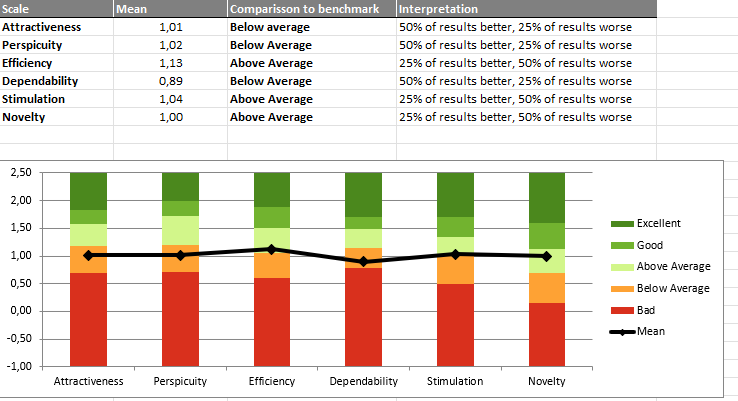
\includegraphics[width=0.8\textwidth]{img/ueq_benchmark.png}
\caption{Hasil Komparasi Benchmark UEQ}
\label{fig:ueq_benchmark}
\end{figure}

Tujuan komparasi data \textit{benchmark} ini adalah untuk mengevaluasi kualitas pengalaman pengguna platform \gls{digilib} IIB Darmajaya berdasarkan standar global yang berisi komparasi dari 21.175 responden terhadap 468 studi produk perangkat lunak (seperti aplikasi bisnis, halaman web, dan jejaring sosial). Hasil perbandingan ini disajikan pada Tabel \ref{tab:ueq_benchmark}.

\begin{table}[htbp]
\centering
\caption{Hasil Komparasi Benchmark UEQ}
\label{tab:ueq_benchmark}
\begin{tabular}{|p{4.5cm}|c|l|p{6cm}|}
\hline
\textbf{Skala (Scale)} & \textbf{Nilai Rata-Rata (Mean)} & \textbf{Kategori Benchmark} & \textbf{Interpretasi} \\ \hline
Daya Tarik (\textit{Attractiveness}) & 1,01 & Below Average & 50\% produk lain lebih baik, 25\% lebih buruk \\ \hline
Kejelasan (\textit{Perspicuity}) & 1,02 & Below Average & 50\% produk lain lebih baik, 25\% lebih buruk \\ \hline
Efisiensi (\textit{Efficiency}) & 1,13 & Above Average & 25\% produk lain lebih baik, 50\% lebih buruk \\ \hline
Ketepatan (\textit{Dependability}) & 0,89 & Below Average & 50\% produk lain lebih baik, 25\% lebih buruk \\ \hline
Stimulasi (\textit{Stimulation}) & 1,04 & Above Average & 25\% produk lain lebih baik, 50\% lebih buruk \\ \hline
Kebaruan (\textit{Novelty}) & 1,00 & Above Average & 25\% produk lain lebih baik, 50\% lebih buruk \\ \hline
\end{tabular}
\end{table}

Berdasarkan Tabel \ref{tab:ueq_benchmark} dan evaluasi \textit{benchmark} di atas, persepsi pengguna terhadap daya tarik (\textit{attractiveness}) berada pada kategori \textit{below average}, menandakan desain antarmuka \gls{digilib} dirasa belum cukup menarik secara visual, di mana 50\% produk sejenis di pasaran memiliki nilai yang lebih baik. Dimensi kejelasan (\textit{perspicuity}) dan ketepatan (\textit{dependability}) juga termasuk dalam kategori \textit{below average}. Hal ini mencerminkan bahwa pengguna masih mengalami kebingungan dalam menavigasi struktur antarmuka serta kurangnya kepercayaan terhadap keandalan sistem saat memproses pencarian atau pemuatan dokumen.

Sementara itu, efisiensi (\textit{efficiency}) dinilai \textit{above average} (di atas rata-rata), menunjukkan bahwa sistem dapat memfasilitasi pengguna untuk menyelesaikan tugas pencarian dengan waktu yang cukup efisien. Dimensi stimulasi (\textit{stimulation}) dan kebaruan (\textit{novelty}) juga berada pada kategori \textit{above average}, mengindikasikan bahwa \gls{digilib} ini secara fungsional dinilai memiliki konsep yang mendukung, inovatif, dan relevan dengan kebutuhan, meskipun eksekusi desain interaksinya masih memunculkan hambatan pragmatis.

\section{Hasil Wawancara}
Untuk memvalidasi dan melengkapi data kuantitatif \gls{ueq}, dilakukan wawancara mendalam dengan perwakilan mahasiswa sebagai pengguna \gls{digilib} IIB Darmajaya. Berdasarkan hasil wawancara, ditemukan beberapa keluhan spesifik yang berbanding lurus dengan rendahnya nilai \textit{dependability} dan \textit{perspicuity}.

Mayoritas narasumber mengeluhkan tata letak (\textit{layout}) halaman pencarian yang terlalu padat, kaku, dan tidak mengelompokkan kategori koleksi referensi secara jelas. Selain itu, sistem filter pencarian dinilai kurang presisi (\textit{dependability} rendah), di mana kata kunci yang dimasukkan pengguna seringkali menampilkan hasil dokumen yang tidak relevan. Dari segi \textit{attractiveness}, pengguna menilai antarmuka terkesan monoton dan tidak diperbarui sesuai standar \gls{ui} modern. Meskipun kecepatan respons sistem dinilai baik, alur navigasi yang berbelit-belit memaksa mahasiswa harus melalui terlalu banyak tahapan (\textit{clicks}) hanya untuk menemukan dan mengunduh satu dokumen yang dituju.

\section{Pembahasan}
Berdasarkan hasil pengujian, evaluasi antarmuka pada aplikasi \gls{digilib} IIB Darmajaya menunjukkan bahwa pengalaman pengguna secara menyeluruh masih jauh dari titik optimal. Dominasi kategori penilaian di bawah rata-rata (\textit{below average}) pada aspek pragmatis maupun visual---terutama \textit{Dependability} (0,89), \textit{Attractiveness} (1,01), dan \textit{Perspicuity} (1,02)---menjadi indikator kuat bahwa sistem saat ini masih memberikan beban kognitif (\textit{cognitive load}) yang tinggi bagi pengguna. Hal ini menuntut adanya perombakan desain yang harus berfokus pada perbaikan arsitektur informasi, penyederhanaan alur interaksi (\textit{user flow}), serta perbaikan algoritma penyaringan data agar hasil pencarian literatur menjadi lebih akurat.

Meskipun aspek \textit{efficiency}, \textit{stimulation}, dan \textit{novelty} menunjukkan hasil \textit{above average}, angka tersebut masih merujuk pada rentang evaluasi yang netral menuju positif ringan (skor 1,00 - 1,13). Angka ini belum mencapai rentang optimal (kategori \textit{good} atau \textit{excellent}). Temuan penelitian ini menegaskan bahwa untuk meningkatkan utilitas dan intensitas penggunaan \gls{digilib} sebagai sumber utama referensi akademik mahasiswa, pengelola sistem tidak cukup hanya mempertahankan stabilitas \textit{back-end} atau server. Diperlukan komitmen untuk menerapkan pendekatan \textit{User-Centered Design} (UCD) pada \textit{front-end} aplikasi agar ekosistem digital kampus menjadi lebih ramah pengguna, intuitif, dan secara langsung berdampak positif terhadap kepuasan layanan sivitas akademika.
\chapter{Kesimpulan dan Saran}\label{cha:conclusion}

\section{Kesimpulan}
Berdasarkan hasil penelitian dan pembahasan mengenai evaluasi pengalaman pengguna pada platform \gls{digilib} IIB Darmajaya menggunakan metode \gls{ueq}, dapat ditarik beberapa kesimpulan sebagai berikut:
\begin{enumerate}
    \item Kualitas pengalaman pengguna (\gls{ux}) pada \gls{digilib} IIB Darmajaya secara keseluruhan masih berada di bawah rata-rata (\textit{below average}) untuk aspek \textit{Dependability} (0,89), \textit{Attractiveness} (1,01), dan \textit{Perspicuity} (1,02). Hal ini menunjukkan bahwa antarmuka sistem masih dirasa membingungkan, kurang menarik secara visual, alur pencarian berbelit-belit, dan filter pencarian kurang presisi.
    \item Beberapa aspek fungsionalitas dan motivasi telah dinilai di atas rata-rata (\textit{above average}), yaitu aspek \textit{Efficiency} (1,13), \textit{Stimulation} (1,04), dan \textit{Novelty} (1,00). Temuan ini menunjukkan bahwa sistem memiliki kecepatan respons yang baik dan konsep fungsional yang cukup inovatif serta relevan dengan kebutuhan mahasiswa.
    \item Hasil dari kuesioner kuantitatif didukung oleh temuan kualitatif melalui wawancara, di mana pengguna mengeluhkan antarmuka yang monoton, tata letak yang terlalu padat, serta filter pencarian yang sering kali menampilkan dokumen tidak relevan.
\end{enumerate}

\section{Saran}
Berdasarkan kesimpulan di atas, beberapa saran konstruktif yang diusulkan untuk pengembangan platform \gls{digilib} IIB Darmajaya di masa depan adalah:
\begin{enumerate}
    \item Menerapkan pendekatan \textit{User-Centered Design} (UCD) pada pengembangan bagian depan (\textit{front-end}) aplikasi untuk menyederhanakan alur navigasi (\textit{user flow}) dan mengurangi beban kognitif pengguna.
    \item Melakukan desain ulang tata letak antarmuka agar lebih modern, tidak terlalu padat, dan mengelompokkan kategori referensi secara lebih jelas dan terstruktur.
    \item Memperbaiki algoritma mesin pencari dan sistem penyaringan (filter) dokumen agar hasil pencarian literatur menjadi lebih akurat dan relevan dengan kata kunci yang dimasukkan pengguna.
\end{enumerate}

\bibliography{ref}

\end{document}
